\chapter{Computational Simulation of Optical Pumping}
This section explores optical pumping through a simulation. The substates of the $|F=2\rangle$ state are modelled as they undergo scattering. This simulation was done in Python3, using the numpy, matplotlib, and sklearn libraries for analysis, regressions, and creating figures. Due to the efficiency of the repump laser and the small amount of leakage, the $|F=1\rangle$ state is not considered in this simulation. The simulation explores the trade off between the final purity of the optical pumping process and the amount of photon scattering, which heats the atom cloud. The number of scatters per atom, on average, required to purify the atoms is a central theme of the simulation. As the optical pumping process happens very fast, faster than the time the mechanical shutter can be turned on and off, the final goal of the simulation is to relate the number scatters required per atom to a required detuning rate to both purify a sufficient percent of the atoms and not overheat the sample. This relation happens from the process described in \textbf{Equation 1.16}
\begin{align*}
R_{scatt} = \frac{\Gamma}{2} \frac{\frac{I}{I_{sat}}}{1 + \frac{I}{I_{sat}} + 4 \left( \frac{\delta}{\Gamma}\right)^2 } \tag{1.16}
\end{align*}
Where $\delta$ is the frequency detuning of our laser. 

\section{Building a Model}

The simulation modeled the population of the ground states, the states of interest, by uniformly populating a 5 element list with integers representing the number of Rubidium atoms in the atom cloud that are in a corresponding $M_F$ substate. This uniform distribution is expected at this stage. From there, a function randomly chooses one of these atoms to excite. The atom chosen is random and therefore choosing an atom from a specific $M_F$ substate depends on the relative population of atoms in a particular $M_F$ substate. From there, the atom obeys selection rules. Since the atom is exposed to positive circularly polarized light along its magnetic dipole moment, it will absorb the angular momentum of the photon and will increase its substate, $|F'=3, M'_F = M_F + 1 \rangle$. Once excited, the atom falls back to $F=2$, choosing its $M_F$ substate based off the relative probabilities described by quantum mechanics in \textbf{Figure 1.7}. This process is repeated, keeping track of the atom cloud states and the number of photon scatters. This model is effective in many ways. It can be used to show the relative population of atom substates over time. The relation is between photons scattered and the proportion of the atoms in the trappable $M_F=2$ substate. From there, as heating increases with the number of photons scattered, an intuitive relation is shown between heating and the number of trappable atoms. In addition, the number of scatters required per atom is easily related to the required intensity and frequency detuning through \textbf{Equation 1.16}.

The model is first run on a theoretical cloud of 100 Rubidium atoms as shown in \textbf{Figure 2.1}.



\begin{figure}[h!]
\begin{center}
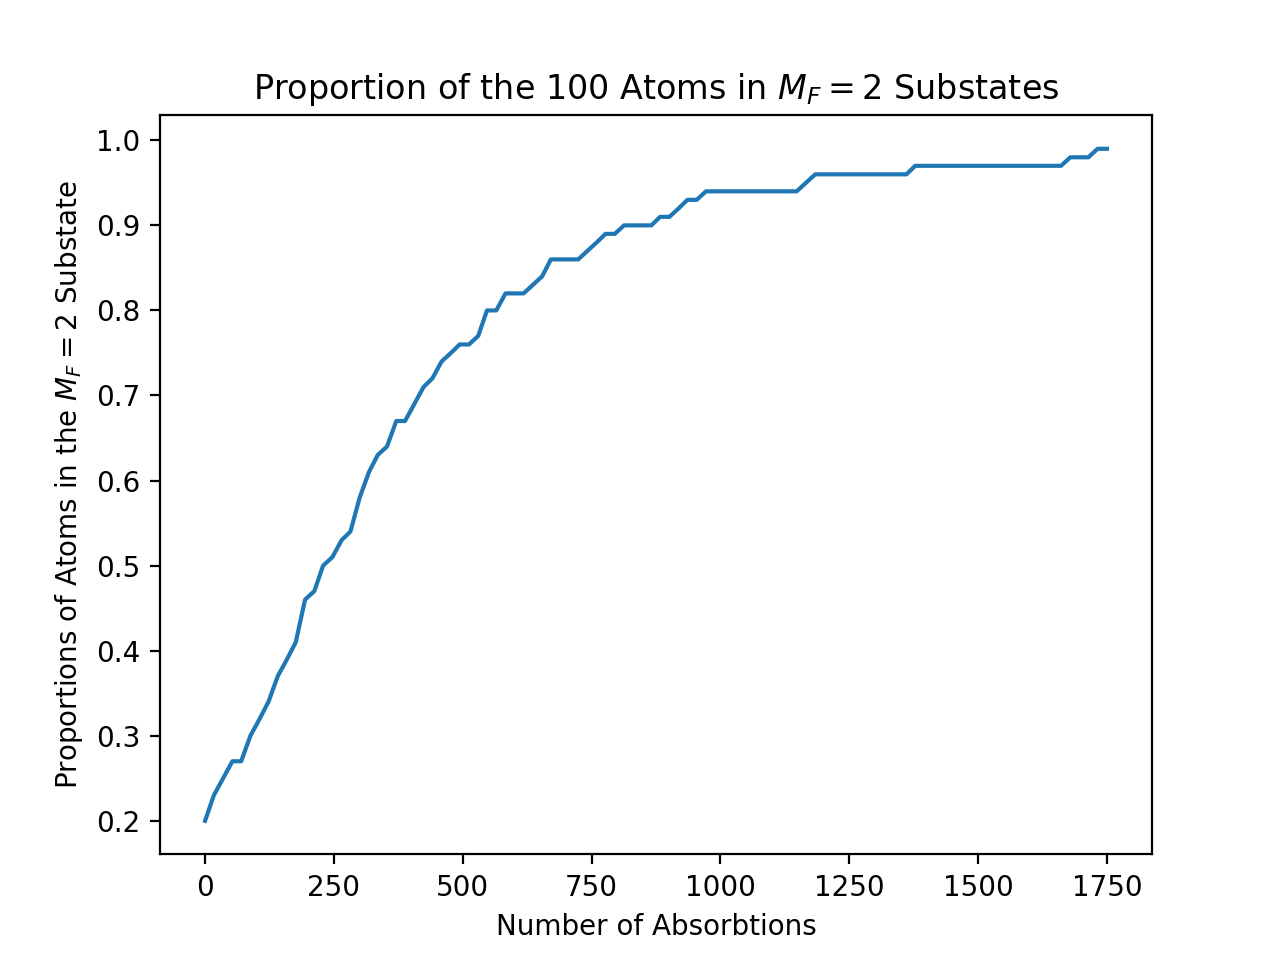
\epsfig{file=fig_prop_atoms_lin.png, scale = .75}
\end{center}
\caption{A visualization of the simulation on a cloud of 100 Rubidium atoms. }
\end{figure}

This figure confirms intuitions on the optical pumping process. Once trapped, atoms do not change their $M_F$ substate, even if they are excited. This is because they will cycle between the $|F=2, M_F=2\rangle$ and $|F'=3, M'_F=3\rangle$ states. It is also clear that getting more atoms in the desired state requires more and more photon scattering as the purity gets high. This is because already trappable atoms start to become scattered more often. This causes unnecessary heating. This can be more accurately viewed in \textbf{Figure 2.2}.

\begin{figure}[h!]
\begin{center}
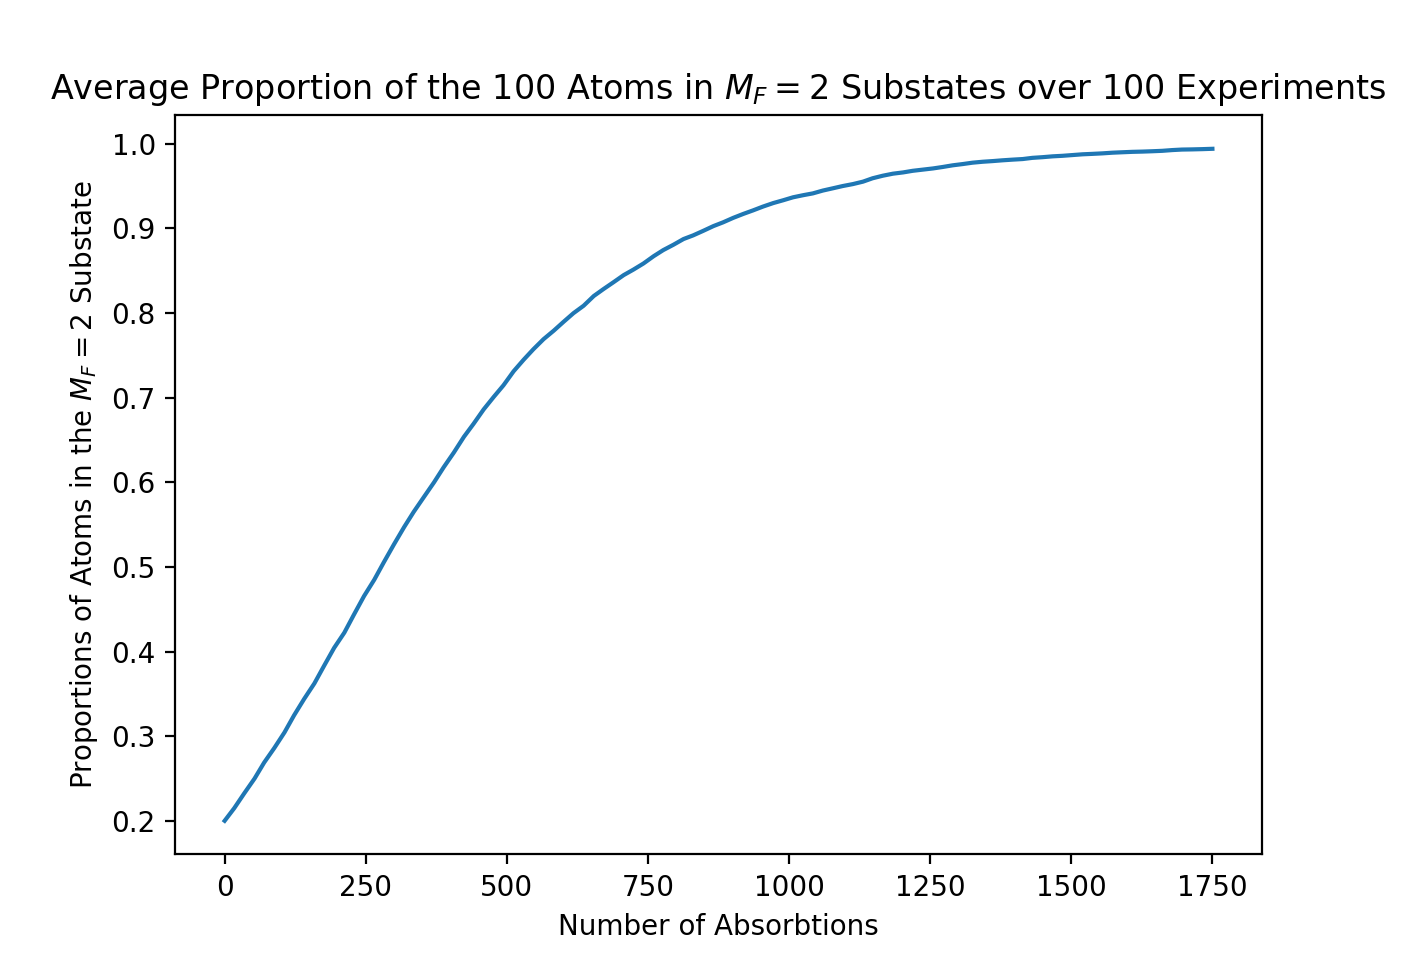
\epsfig{file=fig_avg_lin.png, scale = .75}
\end{center}
\caption{A visualization of the simulation run on a cloud of 100 Rubidium atoms 100 times and averaged. }
\end{figure}

This illustrates the cost-benefit of more photon scattering. At a certain point, achieving a certain purity is no longer desirable as it requires a large amount of scattering and heating of the system. On the NASABEC machine, there are other steps with much higher losses of atoms. While the optical pumping process should be an efficient process, other steps could be optimized if the number of atoms in the Bose-Einstein Condensate is not sufficient. For that reason, the difference between, say, a $95\%$ purity and a $99\%$ purity, is mostly negligible. 
\newline

\section{Scaling the Model}

While this initial model is informative, it cannot be run on a cloud of millions of atoms, like in the lab. The computational requirements are simple too large and could not be completed in time. Nonetheless, the model can be changed to gain intuition on how many photon scatters are required as the atom cloud grows. If a relation can be found between the number of photon scatters and the number of atoms in the purified state, then this relation can be applied to atom clouds with millions of Rubidium atoms. 

To do this, the simulation models how many photon scatters are required to get to a given purity level. The different purity levels explored are $80\%$, $90\%$, $95\%$, and $99\%$. $50$ different atom cloud sizes are explored with each of these purity levels. The atom cloud sizes are linearly distributed from $100$ to $50000$. The simulation takes note of how many photon scatters were required to get each atom cloud to the different purity level. The results for these purity levels are shown below in \textbf{Figure 2.3}.

\begin{figure}[h!]
\begin{center}
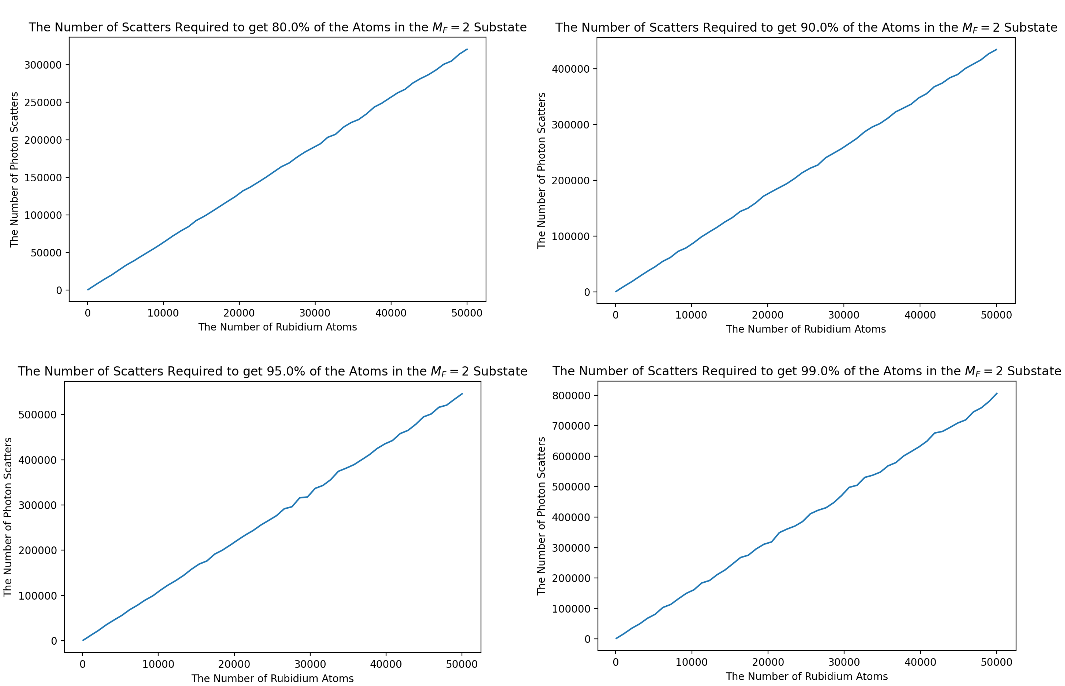
\epsfig{file=fig_many_scatters.png, scale = .45}
\end{center}
\caption{Visualizations of the amount of photon scatters required to trap different percentages of the Rubidium atoms. }
\end{figure}

These graphs show that getting a higher purity level for a given number of atoms requires significantly more scattering and heating. It is also clear from these graphs that the relationship between the number of photon scatters required to purify the atoms and the number of initial atom is linear. This leads to the conclusion that the number of photon scatters required per atom is independent of the number of atoms. This makes sense as, on average, any individual atom has an equal probability of being in any state and the number of scatters required to give the atom a particular probability of being in the trappable state is independent of the amount of Rubidium atoms. This conclusion also makes it possible to model how many scatters are required to purify an atom cloud with millions of atoms. The next step is to determine how many photon scatters is required per atom to get a given purity level. To do this, each of these plots is linearly regressed using a least-squares method. The estimated slope of this regression is the number of photon scatters required per Rubidium atom at the given desired purity level. These regressions are shown below in \textbf{Figure 2.4}.

\begin{figure}[h!]
\begin{center}
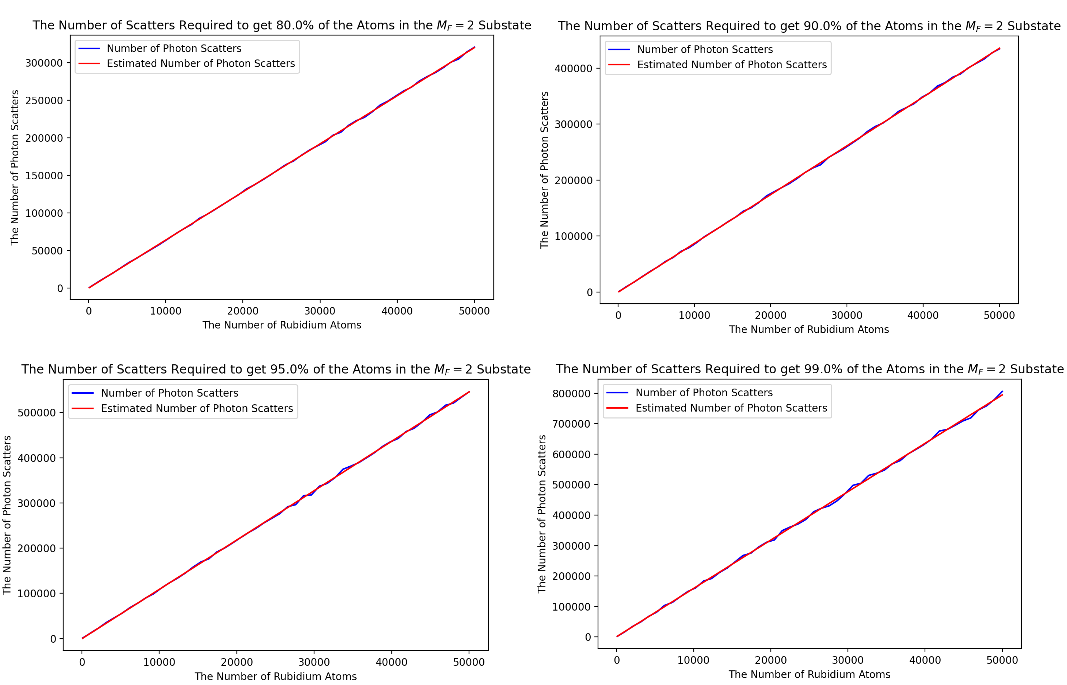
\epsfig{file=fig_many_scatters_reg.png, scale = .45}
\end{center}
\caption{Visualizations of the amount of photon scatters required to trap different percentages of the Rubidium atoms with a least-squares linear regression. }
\end{figure}

For each of these regressions, the coefficient of determination was greater than $99.9\%$, which agrees with the interpretation that the required photon scatters per atom is independent of the number of atoms. The calculated required photons scatterings for each of these experiments is shown in \textbf{Table 1}. 
\begin{table}[h]
\begin{center}
\begin{tabular}{|l|l|r|l|}
\hline
Percent of Atom in the $M_F=2$ State & Photon Scatters per RB Atom\\
\hline
80 & 6.41\\
\hline
90 & 8.72\\
\hline
95 & 10.92 \\
\hline
99 & 15.88 \\
\hline
\end{tabular}
\caption{The amount of scatters required per atom grows as the desired number of atoms in the $M_F=2$ trappable states grows.}
\end{center}
\end{table}

This gives some very accurate results for these purity levels. The amount of scatters per atom grows at an increasing rate. These numbers provide a good opportunity to make a decision of the desired purity levels. While the jump between $90\%$ and $95\%$ purity only requires a $25\%$ increase in the number of scatters, the jump between $95\%$ and $99\%$ requires a $45\%$ increase in the number of scatters. This significantly heats the sample for only $4\%$ more of the original atoms. For that reason, it will be decided that the purity level should be $95\%$. If that sounds low, recall that on other steps of the cooling process, much higher proportions of atoms are lost. Optimizing these steps would be significantly more beneficial to increasing the atom count of the Bose-Einstein Condensate. If that sounds high, it is worth noting that the optical pumping process is typically an efficient step in the process of making a Bose-Einstein Condensate. 

To further study the relation between the number of scatters required for a given purity, one more simulation was performed. This simulation explored more desired purities from $80\%$ to $99\%$. As the previous simulations took hours to run, the atom cloud size had to be greatly reduced. The atom cloud sizes studied for this experiment ranged from $1000$ to $5000$ atoms. Nonetheless, the same general trend can be extracted: the amount of photon scattering per atom grows as the desired purity level grows. 

\begin{figure}[h!]
\begin{center}
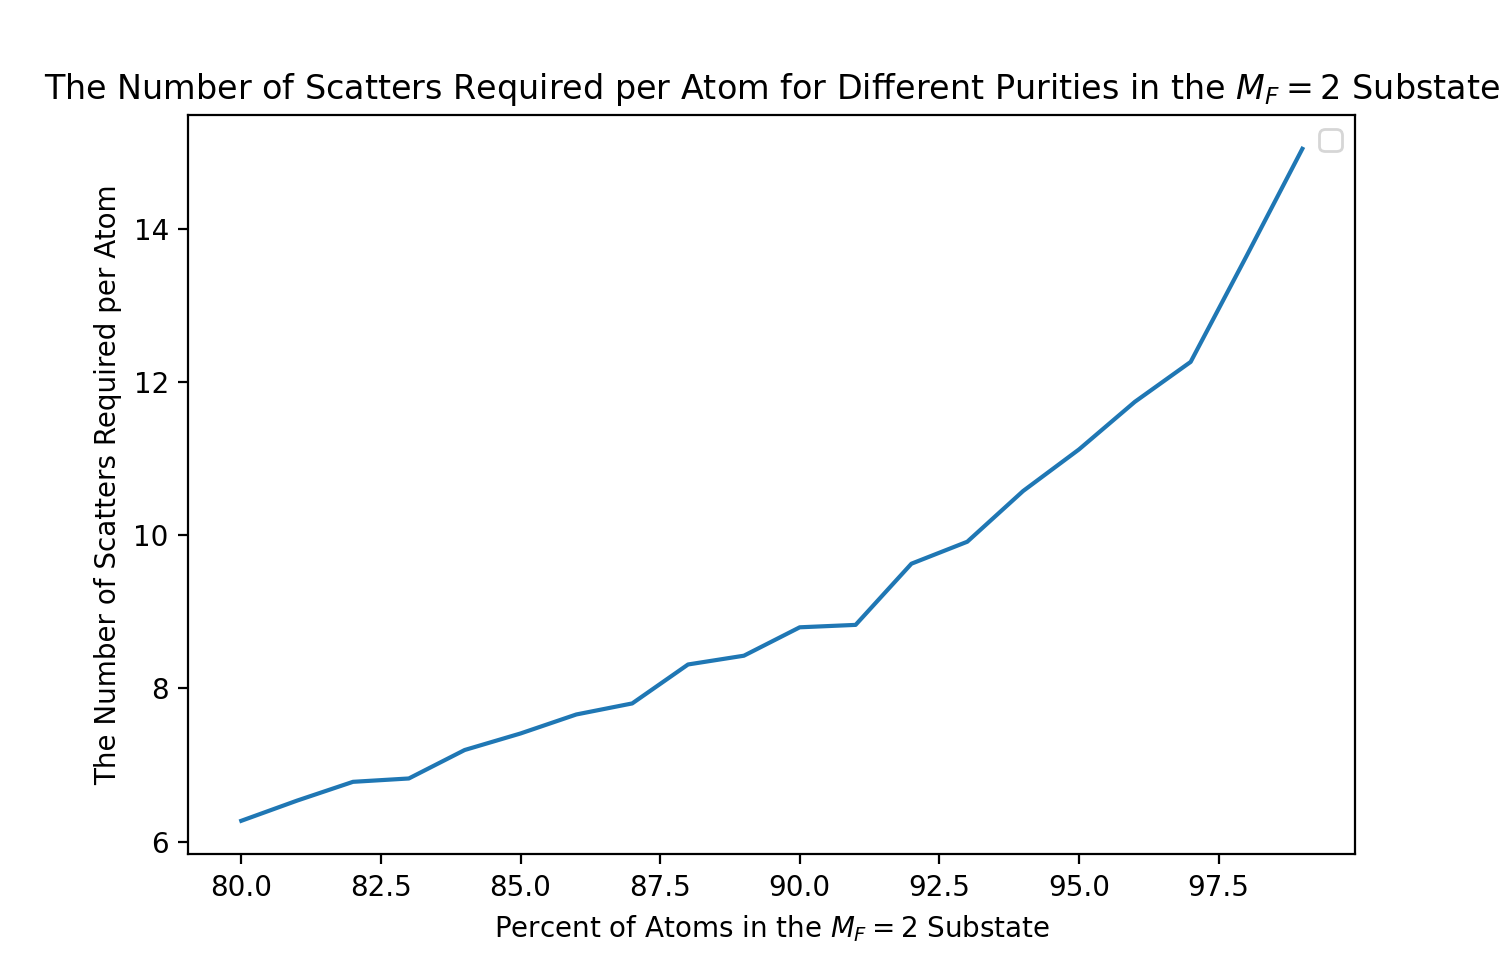
\epsfig{file=fig_scatt_purity.png, scale = .65}
\end{center}
\caption{The amount of scatters required per atom grows seemingly exponentially as the desired number of atoms in the $M_F=2$ trappable states grows. }
\end{figure}

The trade-off of the optical pumping process could be viewed in a different way. A higher purity, which results in more heating, requires more atoms to be lost in the evaporative cooling stage to form a Bose-Einstein Condensate. On the other hand, a lower purity does result in less heating but leaves less atoms to form the Bose-Einstein Condensate. As the final goal is to have the most atoms in our Bose-Einstein Condensate, there is a 'sweet-spot' here to be reached. 
\newline

\section{Calculating a Detuning Frequency}
As stated previously, the NASABEC machine will initially seek an optical pumping efficiency of $95\%$. To do this, each atom must, on average, be scattered by $10.92$ photons. \textbf{Equation 1.16}, which describes the scattering rate per atom at a given intensity and frequency detuning, can be used to calculate the parameters for which our laser must be set. Recall that this process typically happens very fast, faster than the mechanical shutter can open and close to allow the process to happen. Though the intensity could be changed in the lab, a fixed power will be assumed of about $4.75 mW$ leaving the optical fiber cable, as currently set up. Should this be changed, the calculation for the frequency detuning remains simple, knowing that each atom must scatter $10.92$ photons on average. In addition, another purity level can be chosen, and the calculations remain simple. Still, it is recommended to choose a purity level given in \textbf{Table 1} as these values were averaged over a large range of atom cloud sizes. 

\textbf{Equation 1.16} can be related to the number of scatters per atom by multiplying by the time the laser is shone on the atoms, $t_s$
\beq
10.9 = R_{scatt} t_s
\eeq
Substituting in \textbf{Equation 1.16} and solving:

\begin{equation}
        \begin{aligned}[b]
            10.9 &= R_{scatt} t_s\\
            10.9 &=  \frac{\Gamma}{2} \frac{\frac{I}{I_{sat}}}{1 + \frac{I}{I_{sat}} + 4 \left( \frac{\delta}{\Gamma}\right)^2 }t_s\\
            \frac{\delta}{\Gamma} &= \pm \sqrt{\frac{\Gamma\frac{I}{I_{sat}}t_s}{10.9*8} - \frac{1}{4} - \frac{1}{4}\frac{I}{I_{sat}}}
        \end{aligned}
\label{eqn2.qo}
\end{equation}
\beq
\delta = \delta(I, t_s) = \pm \sqrt{\frac{\Gamma\frac{I}{I_{sat}}t_s}{10.9*8} - \frac{1}{4} - \frac{1}{4}\frac{I}{I_{sat}}}\ \Gamma
\eeq
The two solutions mean that the laser can be red or blue detuned and the result will be the same. In this case, for driving the $|F=2\rangle \rightarrow |F'=3\rangle$ transition with $\sigma^+$ light, the saturation intensity is $I_{sat} = 1.669 mWcm^{-2}$ and the natural linewidth is $\Gamma = 38.11 * 10^6Hz$. The time the atoms will be exposed to this light is assumed to be $1.5$ milliseconds. 

To calculate the detuning frequency, the intensity of the light at the atoms must be calculated. The power of the linearly polarized light coming out of the optical fiber cable is $4.75 mW$. The efficiency of a quarter-wave plate, to make the light positive circularly polarized was measured to be $90\%$. As there is no culminating lens attached to the end of the optical fiber, this beam spreads significantly. To calculate the intensity that the atoms see, which is $15.5cm$ away from the optical fiber, two different distances and beam diameters were measured. It was assumed that the beam spread in a cone-like shape over this short distance. The intensity of the light at the atom was calculated to be about $1.669 mWcm^{-2}$. Using this intensity, the necessary frequency detuning can be calculated. 

\beq
\delta(I = 1.669 mWcm^{-2}, t_s = 1.5ms) =\pm 6.9\Gamma = \pm260 MHz
\eeq

The Doppler effect is neglected for this detuning as, on average, its result is zero. As the lasers are typically red detuned for optical pumping, the laser NASABEC machine should be red detuned $260 MHz$ to reach a $95\%$ purity of atoms in the $M_F=2$ trappable substate with our current laser parameters. This result is in agreement with another lab that uses a similar setup and has a frequency detuning of about $230 MHz$. Finally, it is worth noting that this model does not include the fact that the intensity of the laser could decrease across the atom cloud because the number of atoms is relatively small, so this effect is negligible. 

The code used in this section can be found in the \textbf{Appendix}. The main application of this program is to get an estimated required number of photon scatters per atom for a desired purity. After this value is calculated, \textbf{Equation 2.3} describes the relationship between the frequency detuning, laser intensity at the atoms, and the time the laser is to be pumping the atoms. Reiterating, should any of the laser parameters require changing (intensity, frequency detuning, or time pumping) this can easily done through \textbf{Equation 2.3}. 

%% in the other 
